\section{Iterator}

Iterator is a design pattern used to get access to the elements of a collection in an object sequentially without the need to know or expose its underlying representation.

% Description of the design pattern

\subsection*{Example}

Figure~\ref{fig:iterator} presents the UML diagram for the iterator pattern in the project \textit{jsecurity}. In the diagram, \texttt{SimplePrincipalCollection} plays the role of the internal design of the iterator, while the \texttt{DelegatingSubject} is the security layer that handles the collection and other interfaces that extend the collections without exposing all elements of the collection. 

\begin{figure}[htb]
    \centering
    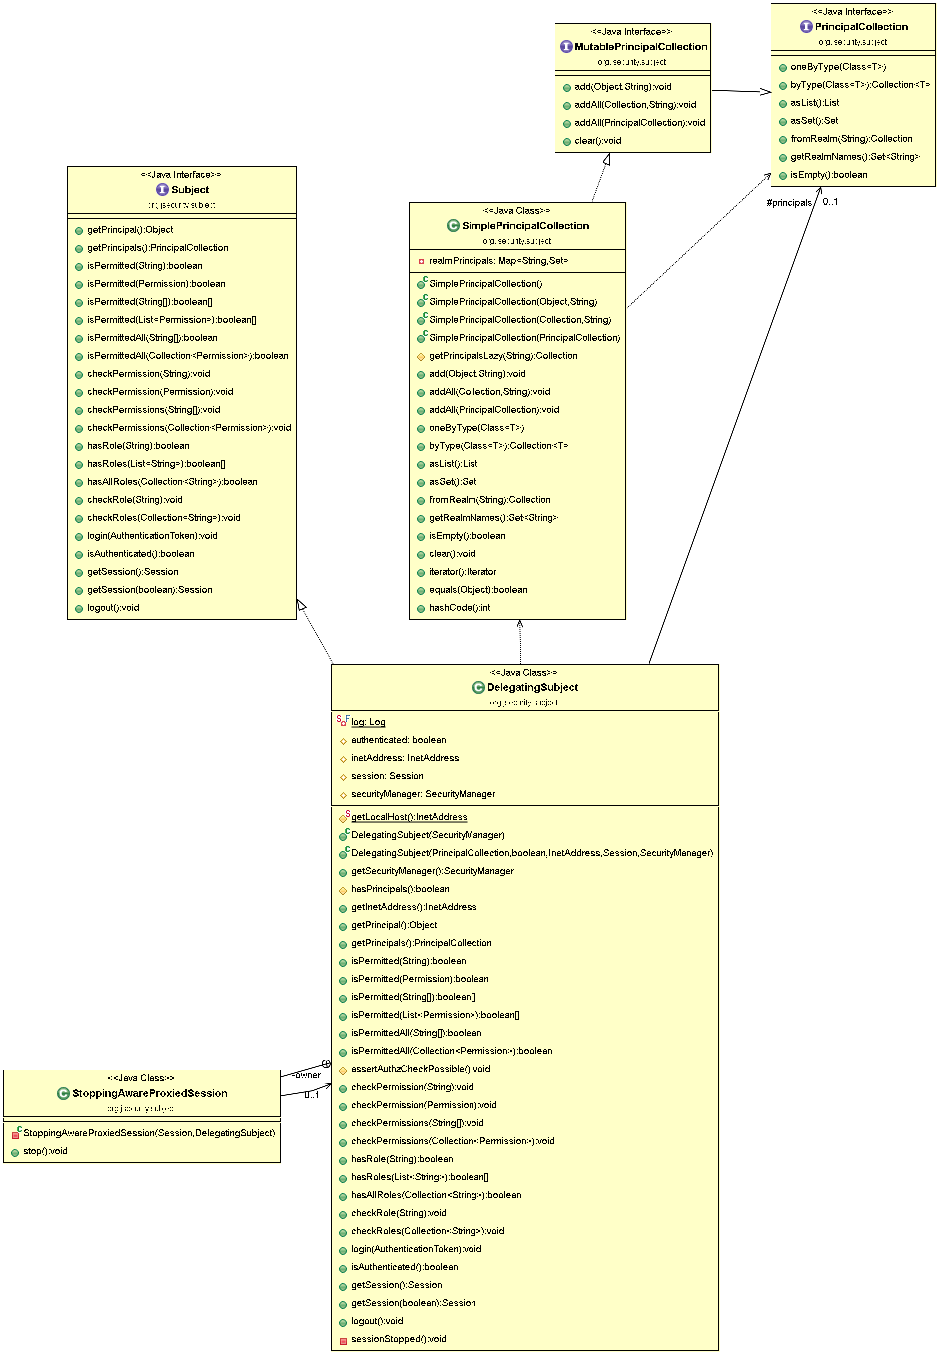
\includegraphics[width=\columnwidth]{images/iterator.png}
    \caption{Iterator design pattern in the project \textit{jsecurity}}
    \label{fig:iterator}
\end{figure}
\FloatBarrier

Figure~\ref{fig:SimplePrincipalColletion} shows the source code of the class \texttt{SimplePrincipalCollection} that implements the \texttt{MutablePrincipalCollection}, in which they implement an internal design of the iterator for the collection.

\begin{figure}[htb]
\centering
\lstset{language=Java, basicstyle=\scriptsize, stepnumber=1, showspaces=false, showstringspaces=false,breaklines=true}
\begin{lstlisting}

public class SimplePrincipalCollection implements MutablePrincipalCollection {

    private Map<String, Set> realmPrincipals;
    public SimplePrincipalCollection() {}

    public SimplePrincipalCollection(Object principal, String realmName) {
        if (principal instanceof Collection) addAll((Collection) principal, realmName);
        } else { add(principal, realmName); }
    }
    public SimplePrincipalCollection(Collection principals, String realmName) {addAll(principals, realmName);}

    protected Collection getPrincipalsLazy(String realmName){
        if (realmPrincipals == null) {
            realmPrincipals = new LinkedHashMap<String, Set>();
        }
        Set principals = realmPrincipals.get(realmName);
        if (principals == null) {
            principals = new LinkedHashSet();
            realmPrincipals.put(realmName, principals);
        }
        return principals;
    }
    public void add(Object principal, String realmName) {
        if (realmName == null) {
            throw new IllegalArgumentException("realmName argument cannot be null.");
        } if (principal == null) {
            throw new IllegalArgumentException("principal argument cannot be null.");
        } getPrincipalsLazy(realmName).add(principal);
    }
    public void addAll(Collection principals, String realmName) {
        if (realmName == null) {
            throw new IllegalArgumentException("realmName argument cannot be null.");
        }
        if (principals == null) {
            throw new IllegalArgumentException("principals argument cannot be null.");
        }
        if (principals.isEmpty()) {
            throw new IllegalArgumentException("principals argument cannot be an empty collection.");
        }
        getPrincipalsLazy(realmName).addAll(principals);
    }
    public void addAll(PrincipalCollection principals) {
        if (principals.getRealmNames() != null) {
            for (String realmName : principals.getRealmNames()) {
                for (Object principal : principals.fromRealm(realmName)) {
                    add(principal, realmName);
                }}}}
    public List asList() {
        Set all = asSet();
        if (all.isEmpty()) {return Collections.EMPTY_LIST;}
        return Collections.unmodifiableList(new ArrayList(all));
    }


    public Iterator iterator() { return asSet().iterator(); }
\end{lstlisting}
\caption{[Iterator] SimplePrincipalColletion.java}
\label{fig:SimplePrincipalColletion}
\end{figure}
\FloatBarrier

Figure~\ref{fig:AttributeModelBuilder} presents the implementation of the interface \texttt{MutablePrincipalCollection}. We can see it extends the principal collection adding all the principals to the given collection.

\begin{figure}[htb]
\centering
\lstset{language=Java, basicstyle=\scriptsize, stepnumber=1, showspaces=false, showstringspaces=false,breaklines=true}
\begin{lstlisting}

public interface MutablePrincipalCollection extends PrincipalCollection {

    void add(Object principal, String realmName);

     void addAll(Collection principals, String realmName);

    void addAll(PrincipalCollection principals);

    void clear();
}
\end{lstlisting}
\caption{[Iterator] AttributeModelBuilder.java}
\label{fig:AttributeModelBuilder}
\end{figure}
\FloatBarrier

Figure~\ref{fig:PrincipalCollection} presents the interface \texttt{PrincipalCollection}, that returns the collection info necessary in different functions.

\begin{figure}[htb]
\centering
\lstset{language=Java, basicstyle=\scriptsize, stepnumber=1, showspaces=false, showstringspaces=false,breaklines=true}
\begin{lstlisting}

public interface PrincipalCollection extends Iterable, Serializable {

    <T> T oneByType(Class<T> type);
    <T> Collection<T> byType(Class<T> type);
    List asList();
    Set asSet();
    Collection fromRealm(String realmName);
    Set<String> getRealmNames();
    boolean isEmpty();
}

\end{lstlisting}
\caption{[Iterator] PrincipalCollection.java}
\label{fig:PrincipalCollection}
\end{figure}
\FloatBarrier

The \texttt{DelegatingSubject} class (Figure~\ref{fig:DelegatingSubject}) delegates the method calls and iterates the objects without exposing the whole collection.

\begin{figure}[htb]
\centering
\lstset{language=Java, basicstyle=\scriptsize, stepnumber=1, showspaces=false, showstringspaces=false,breaklines=true}
\begin{lstlisting}

    public DelegatingSubject(PrincipalCollection principals, boolean authenticated, InetAddress inetAddress,
                             Session session, SecurityManager securityManager) {
        if (securityManager == null) {
            throw new IllegalArgumentException("SecurityManager argument cannot be null.");
        }
        this.securityManager = securityManager;
        this.principals = principals;

        this.authenticated = authenticated;

        if (inetAddress != null) {
            this.inetAddress = inetAddress;
        } else {
            this.inetAddress = getLocalHost();
        }
        if (session != null) {
            this.session = new StoppingAwareProxiedSession(session, this);
        }
    }
    public Object getPrincipal() {
        PrincipalCollection principals = getPrincipals();
        if (principals == null || principals.isEmpty()) {
            return null;
        }
        return principals.asSet().iterator().next();
    }

    public PrincipalCollection getPrincipals() {
        return this.principals;
    }

\end{lstlisting}
\caption{[Iterator] DelegatingSubject.java}
\label{fig:DelegatingSubject}
\end{figure}
\FloatBarrier

The \texttt{Subject} interface (Figure~\ref{fig:Subject}) just gets the \texttt{Objects}, the \texttt{PrincipalCollection}, and checks the role of each element.

\begin{figure}[htb]
\centering
\lstset{language=Java, basicstyle=\scriptsize, stepnumber=1, showspaces=false, showstringspaces=false,breaklines=true}
\begin{lstlisting}
public interface Subject {

    Object getPrincipal();
    PrincipalCollection getPrincipals();
    boolean hasAllRoles(Collection<String> roleIdentifiers);
    void checkRole(String roleIdentifier) throws AuthorizationException;
    void checkRoles(Collection<String> roleIdentifiers) throws AuthorizationException;

}
\end{lstlisting}
\caption{[Iterator] Subject.java}
\label{fig:Subject}
\end{figure}
\FloatBarrier

